

\chapter{Implementation} \label{sec:implementation}

\section{System diagram}

Figure \ref{fig:system} can help the reader to gain understanding how each of the materials and methods used as described in Section \ref{sec:mm} fit together.

\begin{figure}[h!]
    \centering
    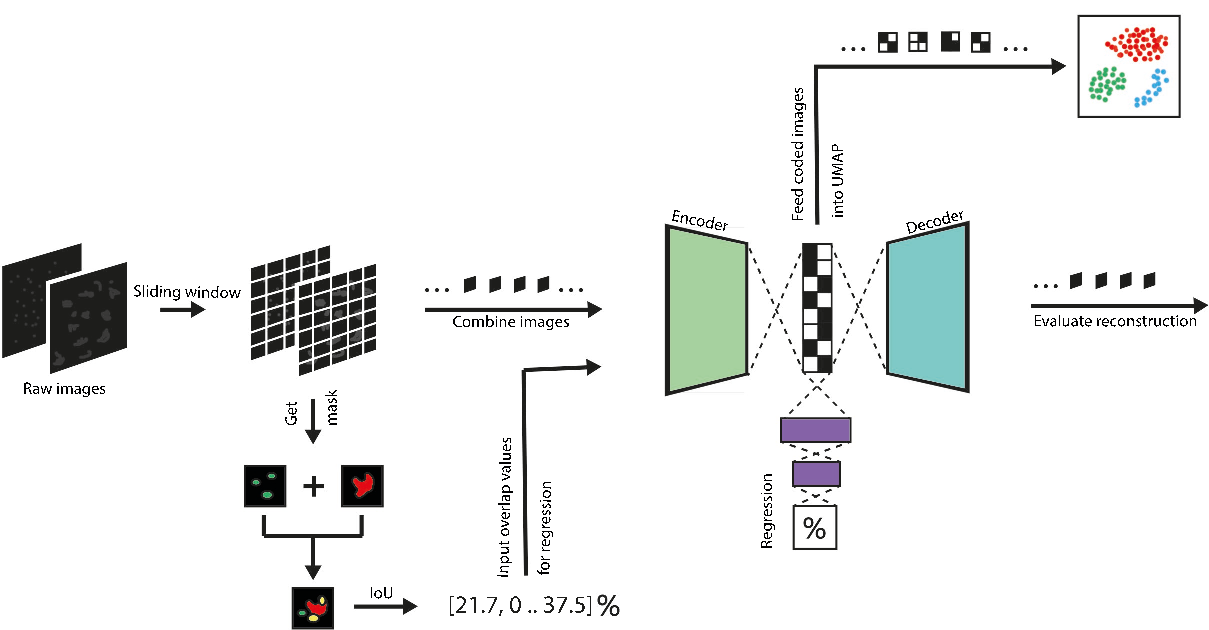
\includegraphics[width=\textwidth]{dissertation/images/system_diagram.jpg}
    \caption{[TODO on Photoshop] System diagram showing how each image will be decomposed and analysed.}
    \label{fig:system}
\end{figure}

\section{Pre-processing}

Firstly, before feeding them as input into any model, the images of cells had to be pre-processed. This is already partly discussed in Section \ref{}. This section will go over some specifics and justify some choices that were made.

\bigskip 
The following list provides a step-by-step of the process:
\begin{enumerate}
    \item For each dataset, all the images of T cells and dendritic cells were picked out. Their corresponding filenames were retrieved.
    \item The filenames were sorted to keep images from the same well next to each other in memory.
    \item Each image was partitioned into sub-images through a sliding window approach. The window was of size 192x192 and yielded a 100 same-sized images. The original image was 2048x2048 so the right and bottom borders of the image were discarded.
    \item Once this gridded dataset was obtained, each T cell image was combined in a RGB image with its dendritic cell counterpart, stored in index i and index i+100 respectively. 
    \item For each combined image, noise was removed through low value pixel clipping. Min-max normalisation was then applied to put all images in the same [0,1] range.
\end{enumerate}

Some choices made in the above have to be justified. 

\subsection{Sliding window}

The sub-image window size was chosen to be 192 because of the pooling and upsampling operations in autoencoders. When an image is processed in the encoder part of the autoencoder, and the 2x2 pooling operations are applied, the image dimensions are reduced by a factor of 2. Each pooling operation has a corresponding upsampling operation in the decoder part of the autoencoder. If a pooling operation results in a decimal dimension, the number is rounded up. The corresponding upsampling operation would then double that number, which would result in a different dimension in the output of the autoencoder. Hence, we had to pick a size that would be big enough to show enough cells, but we also had to pick a size which meant the image could be divided by 2 for a large amount of times, depending on the number of hidden layers. To illustrate, if we apply a division by to the number 200 three times, the image can be upsampled and reconstructed correctly, however if it is reduced 4 times, then after the 4th operation we obtain a 13x13 image and the first upsampling operation creates a 26x26 image. A size which is a multiple of 8 bypasses that issue for a larger number of operations. A 192x192 image can be reduced 6 times, when it reaches dimensions of 3x3, without running into upsampling issues.

\subsection{Image combination}

Images of each type of cells on their own would not make much sense on their own when the aim is to quantify the level of interaction. Hence they have to be combined. The advantage that the provided dataset has is that it comes with the T cells and the dendritic cells separated by means of fluorescent dyes, hence no image segmentation technique had to be used to be able to separate the image out into the different types of cells and colour them in. Instead, each of the T cell and its corresponding DC, which were associated to the same file, were combined together in an RGB image, with the blue channel set to 0. The images were not combined in an absolute difference operation as we would have lost information of where the images overlapped i.e. interacted, which is what we are looking into in this research.

\section{Quantifying immune cell interaction}

To obtain the interaction measure from the images, multiple methods were tried out. Structural Similarity Index was computed, however because the images were so similar in general i.e. white blobs spread across a black background, the results were extremely similar across all cells in different experiment conditions (show image?). The idea was instead to obtain masks of the images and compute the intersection over union area as the interaction value. As the cells were bright blobs on a black background, and we did not have the task of separating T cells from dendritic cells, it was hoped that this would be straightforward. Both K-means and thresholding methods yielded good results.

\subsection{K-means}
K-means has been shown to perform well on colour segmentation. It was easy to initialise. OpenCV's K-means was used over sklearn's because over 1000 images, it performed a lot faster. [recompute] K-means was applied to the images with K=2 and 10 iterations for performance. First, K-means centers were initialised randomly. However, during training and validation it was found that this method of initialisation was yielding highly different results for the intersection over union metric at every run. Hence, some speed was traded for consistency and the kmeans++ center initialisation method was picked instead. 

\subsection{Thresholding}
The alternative to K-means is thresholding. Thresholding depends on pixel value analysis. Usually, thresholding works well for images which have peaks of pixel values in their distribution. However, this was not the case for our images. First, the threshold value picked was the mean pixel value. This yielded acceptable results, however some noisy pixels still came through the mask. 

[illustrate as you write !!!]

To fix that problem, the threshold value was set as the sum of the mean pixel value and the standard deviation. This decision was made on the hypothesis that the noise level of an image with a flat structure can be estimated from its variation.

\subsection{Image masks for background correction}
As mentioned in materials & methods, the images might have noise. Particularly in biomedical data, there has been research on background correction. Rather than fixing the background, we can evaluate whether removing the background entirely helps in this case by evaluating both masked an unmasked images.

\section{Convolutional autoencoder}

The main tool to be developed to exploit this dataset was a convolutional autoencoder. The autoencoder was built for two purposes: obtaining a smaller "code" representing each of the images to be fed into high-dimensional visualisation algorithms, and to be the starting block for a deep regression model.

\subsection{Structure}

The autoencoder was built using Keras \footnote{https://keras.io} for Python. We based our architecture off the standard Convolution --> Activation --> Pooling sequence of operations commonly used in convolutional neural networks (ref). The aim was to maximise the reduction of dimensionality while maintaining a satisfactory reconstructed image. Hence, the choice of number of hidden layers had to be made as a compromise. 

The autoencoder was tuned by evaluation on a training and validation dataset. Its structure was established through both literature review and trial and error. The choice of hidden layer activation is PReLU, because of its evidenced benefit in improved loss (ref), as well as showing slightly better results in training. Moreover, convolutional layer sizes were kept quite high, instead making the neural network deeper to reduce dimension. Strides are used in the last layer instead of max pooling (why?) because results were slightly better. The choice of feature maps being higher in earlier layers comes from the encoded representation being smaller this way, as well as differences with the reversed being marginal. Finally, the output layer activation is sigmoid, as we are trying to predict a value between 0 and 1, as the images have been normalised. 

\subsection{Deep regression}

The regression model was built on the encoder layers of the autoencoder. The structure of the regression layers of the model was kept simple. Only two fully connected layers are used, with a Dropout layer in between. Dropout has shown to make models more robust and prevent overfitting. 
Both softplus and linear activations were tried for the regression model. The linear activation was accompanied with a kernel restriction on the keras model of non-negativity, as interaction cannot be negative. Softplus keeps its output values positive. The results were similar, however the linear function performed overall better.